\section{Protocole 802.1x}
\label{dot1x}
\subsection{Généralités}

Le standard 802.1X permet le contrôle d'accès à un réseau port par port grâce à un serveur RADIUS.

Le principe est décrit sur le schéma suivant :\\
\begin{center}
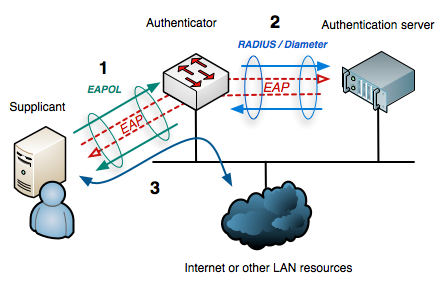
\includegraphics[width=250pt]{img/schema-dot1x.png}\footnote{\url{http://en.wikipedia.org/wiki/IEEE_802.1X}}
\end{center}

Il existe trois rôles :
\begin{enumerate}
\item Le \textit{supplicant} est la partie cliente qui s'occupe de l'authentification.
\item L'\textit{authentificator} correspond au switch. C'est lui qui demande l'authentification du client, formules les requêtes RADIUS et configure l'accès au réseau du client.
\item Le serveur RADIUS est appelé \textit{authentification server}. Il vérifie la validité du client et communique le résultat au switch.
\end{enumerate}

Le standard 802.1X est disponible nativement sur Windows (depuis XP), linux et mac. Il suffit d'avoir un supplicant d'installé.

Le transport des informations est assuré par le protocol EAP. Entre le \textit{supplicant} et l'\textit{authentificator}, il s'agit du protocol EAP over LANs (EAPOL). Et entre l'\textit{authentificator} et le \textit{authentication server}, il s'agit du protocol EAP over RADIUS.

Un port 802.1X a deux rôles logiques :
\begin{enumerate}
\item unauthorized - Aucune trame n'est transmise sauf celle pour l'authentification.
\item authorized - Toute les trames sont transmises normalement.
\end{enumerate}

\subsection{Protocole d'authentification}

Les échanges sont illustrés sur le schéma suivant :\\
\begin{center}
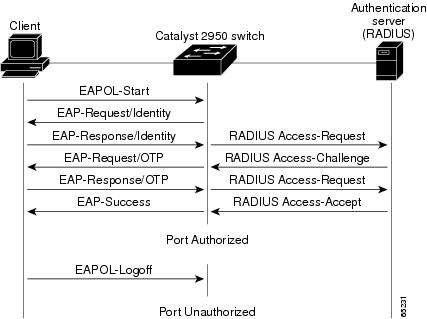
\includegraphics[width=250pt]{img/authentification.jpg}\footnote{\url{http://www.cisco.com/en/US/docs/switches/lan/catalyst2950/software/release/12.1_19_ea1/configuration/guide/Sw8021x.html}}
\end{center}

Les échanges sont décris ci-dessous :\\
\begin{enumerate}
\item A la détection d'un nouveau supplicant, le port s'active et passe en mode unauthorized, seule les trames EAPOL sont autorisées.
\item Puis, l'authentificator envoie régulièrement une EAP-Request Identity à une adresse MAC spécifique. Le supplicant écoute sur cette adrese. Dès qu'il reçoit la EAP-Request Identity, il envoie une EAP-Response Identityavec une information d'identification (comme un User-ID).
\item Dès la réception de la EAP-Response Identity, l'authentificator l'encapsule dans un paquet RADIUS Access-Request et l'envoie à l'authentication server.
\item A tout moment, le supplicant peut réinitialiser la connexion grâce à une trame EAPOL-Start.
\item L' authentification server répond à l'authentificator avec un RADIUS Access-Challenge qui contient une EAP Request qui spécifie la méthode EAP à utiliser. Elle s'approche au maxium de ce que le supplicant désirait.
\item L' authentificator encapsule envoie l'EAP Request au supplicant. Ce dernier accepte en continuant la discussion avec le protocol EAP choisi ou bien refuse en envoyant un NAK ("Negative Acknowledgement") 
\item Si l'authentification server et le supplicant sont d'accord sur la méthode EAP, l'échange se poursuit entre ces deux entités (relayé par l'authentificator) jusqu'à ce que l'authentification server envoie un message  EAP-Success encapsulé dans un paquet RADIUS Access-Accept ou un message  EAP-Failure encapsulé dans un paquet  RADIUS Access-Reject.
\item Si l'authentification est réussie, l'authentificator met son port en mode authorized et le trafic normal est autorisé, sinon le port reste en mode unauthorized
\item Pour se déconnecter, le supplicant envoie un message EAPOL-logoff ce qui a pour conséquence de mettre le port en mode unauthorized.
\end{enumerate}

\subsection{Configuration Cisco}
\subsubsection{Activer le 802.1X sur le switch}

\begin{verbatim}
Switch(config)# aaa new-model
Switch(config)# aaa authentication dot1x default group radius
Switch(config)# dot1x system-auth-control
\end{verbatim}

\subsubsection{Reset et paramètres par défaut}

Pour réinitialiser la configuration du 802.1X sur le switch :

\begin{verbatim}
Switch(config)# dot1x default
\end{verbatim}

La configuration par défaut est :
\begin{itemize}
\item Authentication, authorization, and accounting (AAA) authentication <-> Disable
Disabled. 
\item RADIUS server : IP address <-> None specified
\item RADIUS server : UDP authentication port <-> 1812
\item RADIUS server : Key <-> None specified
\item Per-interface 802.1X enable state <-> Disabled (force-authorized)
\item Periodic re-authentication <-> Disabled
\item Number of seconds between re-authentication attempts <-> 3600 seconds
\item Quiet period <-> 60 seconds
\item Retransmission time <-> 30 seconds
\item Maximum retransmission number <-> 2 times
\item Multiple host support <-> Disabled
\end{itemize}

\subsubsection{Configurer une interface}

\begin{verbatim}
Switch(config)# interface fastethernet0/1
Switch(config-if)# dot1x port-control {auto | force-authorized | force-unauthorized}
\end{verbatim}

\subsubsection{Incompatibilités}

La fonctionnalité 802.1X ne peut être activée sur les ports :
\begin{enumerate}
\item Trunk
\item Dynamic
\item Dynamic-access
\item Etherchannel
\item Secure
\item Switch Port Analyzer (SPAN)
\end{enumerate}

\subsubsection{Authentification périodique}

\begin{verbatim}
Switch(config)# dot1x re-authentication
Switch(config)# dot1x timeout re-authperiod 4000
\end{verbatim}

\subsubsection{Période entre 2 tentatives de connexions}

\begin{verbatim}
Switch(config)# dot1x timeout quiet-period 30
\end{verbatim}

\subsubsection{Période entre 2 paquets EAP Request/Identity}

\begin{verbatim}
Switch(config)# dot1x timeout tx-period 60
\end{verbatim}

\subsubsection{Nombre maximum de paquets EAP Request/Identity}

\begin{verbatim}
Switch(config)# dot1x max-req 5
\end{verbatim}

\subsubsection{Plusieurs 'Host' sur une seule interface}

\begin{verbatim}
Switch(config-if)# dot1x multiple-hosts
\end{verbatim}

Note : Un host identifié donne accès au réseau à tous les autres. Un host qui se déconnecte bloque l'accès à tous les autres.

\subsubsection{Débuguer}

\begin{verbatim}
Switch(config)# show dot1x
Switch(config)# show dot1x statistics
Switch# debug dot1x all
\end{verbatim}

\subsubsection{VLAN invité}

\begin{verbatim}
Switch(config-if)# dot1x guest-vlan { vlan-id }
\end{verbatim}

\subsection{Failles}

\subsubsection{Attaque de la méthode d'authentification}

\textbf{Dictionnaire hors-ligne avec EAP MD5}

Une attaque par dictionnaire hors-ligne, cette attaque peut se pratiquer contre EAP-MD5 dans le cas ou la communication entre le client et le contrôleur d'accès est non-filaire. 

On procède donc à une écoute de ce qui transite sur le réseau, on peut donc identifier le hash du défi et le défi qui transitent. 

On peut ensuite procéder à une recherche dite "hors-ligne", car on peut essayer de retrouver le mot de passe sans avoir à le soumettre au serveur. 

C'est pourquoi il est proscrit d'utiliser EAP-MD5 pour du non-filaire. En cas de réseau filaire l'attaque ne pourra pas se faire "hors-ligne", il faudrait soumettre chaque tentative de mot de passe au serveur. 

Cette attaque n'est pas dangereuse si celui-ci refuse, au bout de 3 tentatives en échec, toute nouvelle tentative provenant du même utilisateur pour une durée de 10 minute par exemple. 

\textbf{Dictionnaire en ligne avec EAP PEAP/TTLS}

Le fait de protéger la communication entre le client est le point d'accès par un tunnel crypté est une bonne chose dans le cas ou l'on veut effectuer les authentifications sur du non-filaire.
Cela permet de se prémunir contre les attaques par dictionnaire "hors-ligne", et force les usurpateurs à soumettre leurs requêtes aux serveurs. 
Ces serveurs qui sont comme cité précédemment prévu pour refuser un nombre trop grand de tentative pour un même utilisateur. 

\subsubsection{Attaque de session après connexion}

Le protocole EAP seul ne protège pas la session, le contrôleur d’accès se contente de vérifier que l’adresse MAC à déjà été validé. Une fois l’authentification établie, le trafic entre le contrôleur d'accès et le client n’est pas chiffré. 

Dans le cas d’une communication wifi, il est très facile d'écouter ce qui transite sur le réseau. Une fois l'authentification réalisé il est donc impératif de mettre en place un tunnel chiffré à l’aide de WPA ou WPA2 par exemple. 

Sinon il serait très facile pour un pirate d'écouter la communication, et de récupérer l'adresse MAC du client. Une fois cette adresse MAC trouvée, il pourra se faire passer pour ce client, technique dite du "Spoofing d'adresse MAC". 

\subsubsection{Attaque 'Man in the middle'}

Cette attaque est facile à réaliser dans le cas d’une communication wifi. 

Le pirate peut procéder en créant un point d'accès wifi pirate, qui aurait le même SSID que le point d'accès authentique. 

Une fois qu'un client vient pour s'y connecter, il suffit de procéder à l'authentification avec le vrai point d'accès, en utilisant les valeurs que le client nous envoie. 

\subsubsection{Solutions}

Pour pallier à toutes ces failles on peut effectuer les actions suivantes : 
\begin{itemize}
\item Utiliser en priorité EAP-TLS, EAP-PEAP ou EAP-TTLS. 
\item Mettre en place un tunnel chiffré entre le point d’accès et le client (WPA ou WPA2) dans le cas du wifi. 
\end{itemize}
